% ============================================================
% Q1: Bayesian Inverse Estimation of Latent Fan Vote Shares
% (Academic simplification; ~4 pages target; layout/footnotes streamlined)
% ============================================================

\section{\textbf{Reconstruction of Latent Fan Voting Distribution }  }
\label{sec:q1}

Observed eliminations reveal only partial, order-type information about audience support: the show does not disclose total vote counts nor contestant-level vote allocations. Hence, any downstream mechanism audit must begin with a regime-consistent reconstruction of weekly fan support under the same observability limits. We therefore infer, for each week $(s,t)$, a \emph{posterior distribution} over the simplex of fan vote shares whose implied elimination remains compatible with the historical outcome under the season-specific aggregation rule.

This posterior is the sole admissible interface from Q1 to later questions: it allows (i) controlled counterfactual comparisons of aggregation rules under a common uncertainty budget (Q2), and (ii) evaluation of minimal safety layers whose observables are limited to bottom-group membership (Q3). These are precisely the ingredients required for the Q4 MSN proposal (percent baseline + bottom-two safety + optional fan-facing features), without introducing any unobservable external data.

% ------------------------------------------------------------
% 1. Data interface
% ------------------------------------------------------------
\subsection{Simplex-Based Data Preprocessing and Normalization }
\label{sec:q1_data}

First, to ensure mathematical consistency, we explicitly define the \textbf{Active Contestant Set} $C_{s,t}$ as the subset of contestants with at least one non-missing judge score in week $(s,t)$. This definition ensures that post-elimination placeholders do not artificially distort the normalization process, and all subsequent computations are strictly restricted to $i \in C_{s,t}$.

Next, to standardize heterogeneous judge panels (whose size varies by week), we define each contestant's valid weekly judge score as the mean over \emph{available (non-missing) judges}. Let $\mathcal{J}_{s,t}$ denote the set of judges present in week $(s,t)$ and $S_{j,i,s,t}$ be judge $j$'s score for contestant $i$ (ignoring entries marked as N/A). Then
\[
J_{i,s,t}:=\frac{1}{|\mathcal{J}_{s,t}|}\sum_{j\in\mathcal{J}_{s,t}} S_{j,i,s,t},
\]
which coincides with the cleaned field \texttt{wt\_avg}. We then map judges' input onto the simplex via
\begin{equation}
\mathbf{p}^{J}_{s,t}=\frac{\mathbf{J}_{s,t}}{\mathbf{1}^\top \mathbf{J}_{s,t}}\in\Delta^{|C_{s,t}|-1},
\label{eq:q1_jshare}
\end{equation}
where $\mathbf{J}_{s,t}\in\mathbb{R}_+^{|C_{s,t}|}$ collects $J_{i,s,t}$ for $i\in C_{s,t}$.


\begin{table}[h]
\centering
\small
\setlength{\tabcolsep}{5pt}
\renewcommand{\arraystretch}{1.05}
\caption{\textbf{Regime mapping and admissible observable implications.} Feasibility constraints in Q1 must follow the historical rule in each era.}
\label{tab:q1_regime_map}
\begin{tabular}{lll}
\toprule
Era & Rule family & Observable implication used in Q1 \\
\midrule
Seasons 1--2 & Rank (judge-rank + fan-rank) & $E_{s,t}= \mathrm{Worst}_{m_{s,t}}(\mathbf{B}_{s,t}(\mathbf v_{s,t}))$ \\
Seasons 3--27a & Percent (judge-share + vote-share) & $E_{s,t}=\mathrm{Bottom}_{m_{s,t}}(\mathbf{p}^{J}_{s,t}+\mathbf{v}_{s,t})$ \\
Seasons 28a--34 & Judges' Save layer & $E_{s,t}\subseteq \mathrm{BottomTwo}^{\mathcal{R}(s)}_{s,t}(\mathbf v_{s,t})$ \\
\bottomrule
\end{tabular}
\end{table}

Finally, we derive a critical \textbf{Design Implication} for the optimization phase (Q4). Our analysis suggests that the ``Save Era'' reveals only a bottom-group constraint, which analytically separates a \emph{baseline aggregator} from a \emph{safety layer}. This \textbf{Structural Separation} is directly exploited in our proposed model: we select a stable percent baseline (validated in Q2) and augment it with the weakest verifiable bottom-two protection (analyzed in Q3), reserving specific fan-facing features solely for engagement purposes.

% ------------------------------------------------------------
% 2. Bayesian inverse model
% ------------------------------------------------------------
\subsection{Constrained Posterior Sampling via Dirichlet Priors }
\label{sec:q1_model}

With the observables standardized, we let $\mathbf{v}_{s,t}=(v_{i,s,t})_{i\in C_{s,t}}\in\Delta^{|C_{s,t}|-1}$ denote the \textbf{Latent Fan Vote-Share Vector}. To incorporate the structural relationship between technical merit and popularity, we use a weak \textbf{Dirichlet Prior} centered around a softmax transform of judge shares.
\begin{equation}
\mathbf{v}_{s,t}\sim\mathrm{Dirichlet}(\alpha \mathbf{b}_{s,t}),\qquad 
\mathbf{b}_{s,t}=\mathrm{softmax}(\tau\mathbf{p}^{J}_{s,t}),
\label{eq:q1_prior}
\end{equation}
where $\alpha$ controls concentration and $\tau$ controls the alignment strength with judges.

\paragraph{Momentum prior (cold-start mitigation).}
To avoid cold-start bias from a week-independent prior (e.g., contestants with strong pre-existing fan bases), we re-center the Dirichlet proposal in week $t$ using information from week $t-1$:
\begin{equation}
\mathbf{b}_{s,t}=(1-\lambda)\,\mathrm{softmax}(\beta \mathbf{p}^{J}_{s,t})+\lambda\,\mathcal R_{s,t}(\bar{\mathbf{v}}_{s,t-1}),
\label{eq:q1_momentum_prior}
\end{equation}
where $\lambda\in[0,1]$ controls memory strength, $\bar{\mathbf{v}}_{s,t-1}$ is the posterior mean of week $t-1$, and $\mathcal R_{s,t}(\cdot)$ restricts to $C_{s,t}$ and renormalizes. We set $\lambda=0$ for $t=1$, so Eq.~\eqref{eq:q1_prior} is recovered.


Crucially, the geometry of the solution space is determined by the aggregation mechanism in effect. We define the \textbf{Regime-Specific Feasible Set} $\mathcal{A}_{s,t}$ as the collection of vote shares that reproduce the observed elimination under the historical rule:
\begin{equation}
\mathcal{A}_{s,t}=
\begin{cases}
\{\mathbf{v}_{s,t}:E_{s,t}=\mathrm{Bottom}_{m_{s,t}}(\mathbf{p}^{J}_{s,t}+\mathbf{v}_{s,t})\}, & s\in \text{Percent era},\\
\{\mathbf{v}_{s,t}:E_{s,t}= \mathrm{Worst}_{m_{s,t}}(\mathbf{B}_{s,t}(\mathbf{v}_{s,t}))\}, & s\in \text{Rank era},\\
\{\mathbf{v}_{s,t}:E_{s,t}\subseteq \mathrm{BottomTwo}_{s,t}^{\mathcal{R}(s)}(\mathbf{v}_{s,t})\}, & s\in \text{Save era},
\end{cases}
\label{eq:q1_regimes}
\end{equation}
with $m_{s,t}=|E_{s,t}|$ representing the number of eliminated contestants.


To operationalize Eq.~\eqref{eq:q1_regimes}, we use deterministic set operators. For a vector $\mathbf x\in\mathbb R^{|C_{s,t}|}$, let
\[
\mathrm{Bottom}_{m}(\mathbf x):=\arg\min_{\substack{S\subseteq C_{s,t}\\ |S|=m}}\sum_{i\in S} x_i
\]
denote the indices of the $m$ smallest entries (with ties broken deterministically).

\textbf{Rank era.} Let $R(\cdot)$ be the descending rank operator (rank $1$ is best). Define
$r^J_{i,s,t}=R(J_{i,s,t})$ and $r^F_{i,s,t}(\mathbf v)=R(v_{i,s,t})$ and the rank-sum disadvantage
$B_{i,s,t}(\mathbf v)=r^J_{i,s,t}+r^F_{i,s,t}(\mathbf v)$.
Then
\[
\mathrm{Worst}_{m}(\mathbf B(\mathbf v)) := \arg\max_{\substack{S\subseteq C_{s,t}\\ |S|=m}}\sum_{i\in S} B_{i,s,t}(\mathbf v),
\]
i.e., the $m$ contestants with the \emph{largest} rank sums (worst overall standing).

\textbf{Save era (observable bottom-group constraint).} Let $c_i(\mathbf v)$ denote the baseline composite score implied by the regime label $R(s)$ (Percent or Rank). The observable implication is restricted to bottom-group membership:
\[
\mathrm{BottomTwo}^{R(s)}_{s,t}(\mathbf v):=\mathrm{Bottom}_{2}\!\left(\{c_i(\mathbf v)\}_{i\in C_{s,t}}\right),
\qquad
E_{s,t}\subseteq \mathrm{BottomTwo}^{R(s)}_{s,t}(\mathbf v).
\]
We treat boundary cases (e.g., $m_{s,t}=0$) as non-elimination weeks and do not use them in elimination-based inference.

\begin{equation}
p(\mathbf{v}_{s,t}\mid D_{s,t})\ \propto\ p(\mathbf{v}_{s,t})\cdot \mathbb{I}(\mathbf{v}_{s,t}\in\mathcal{A}_{s,t}),
\label{eq:q1_truncpost}
\end{equation}
where $D_{s,t}$ denotes observables. We approximate this distribution via accept--reject sampling to populate the latent vote database.

% ------------------------------------------------------------
% [FIGURE PLACEHOLDER Q1-F1] Pipeline + accept--reject logic
% Insertion location: immediately after Eq.~\eqref{eq:q1_truncpost}.
% Replaces: the long step-by-step narrative of the accept--reject implementation.
% Data source (symbolic): inputs $(C_{s,t},E_{s,t},\mathbf{J}_{s,t})$; output draws $\{\mathbf v^{(m)}_{s,t}\}_{m=1}^M$.
% Figure attributes: flowchart, left-to-right, 6 boxes; include key equations references.
% ------------------------------------------------------------
\begin{figure}[H]
\centering
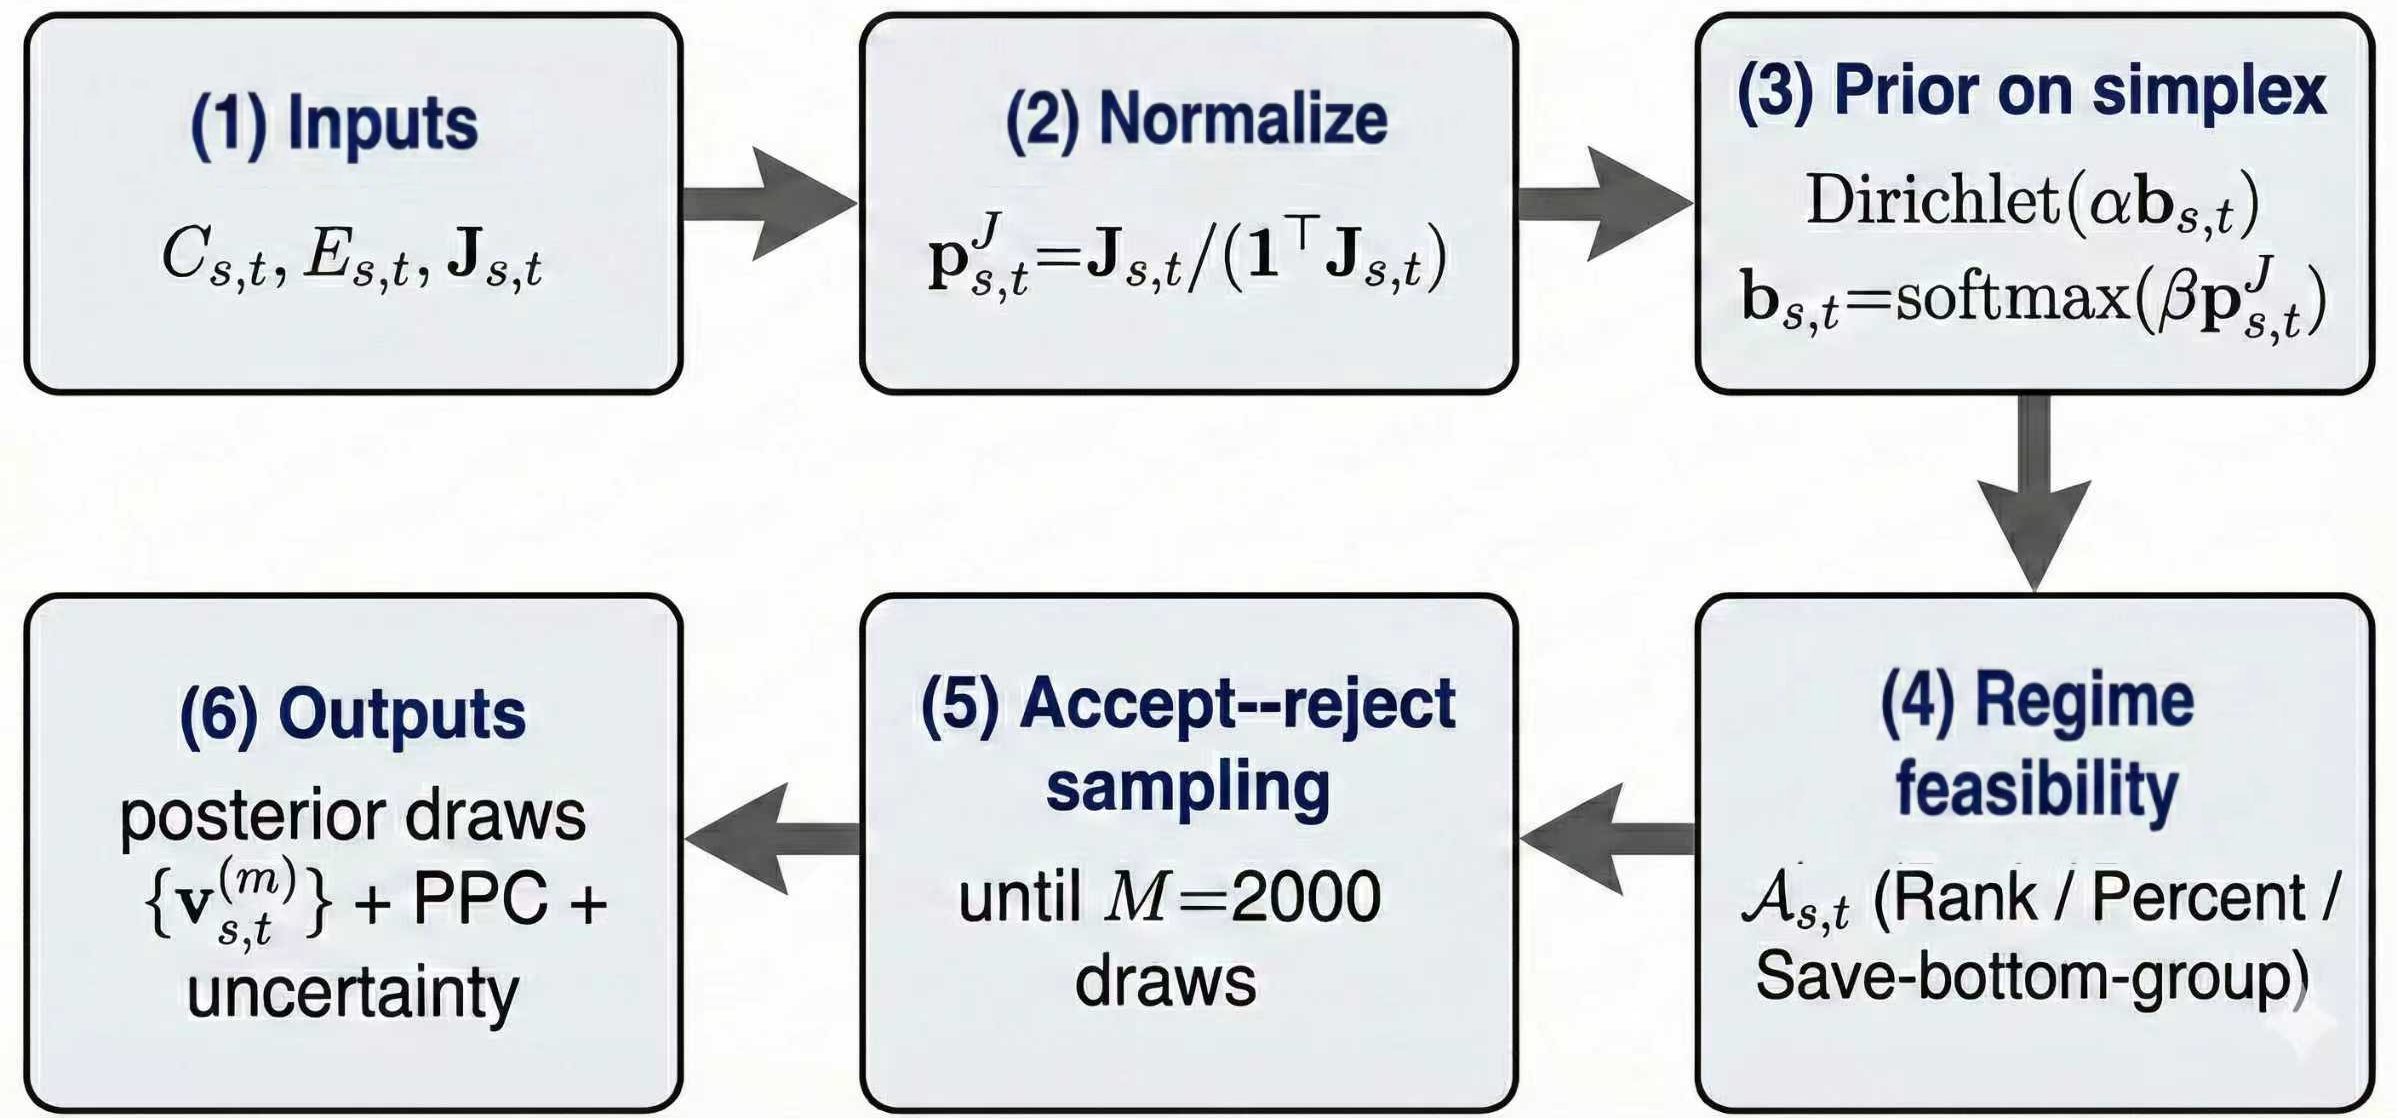
\includegraphics[width=0.52\textwidth]{figures/f1.png}
\caption{\textbf{Q1 pipeline (regime-aware inverse reconstruction).} Weekly inputs $(C_{s,t},E_{s,t},\mathbf{J}_{s,t})$ are mapped to posterior draws $\{\mathbf v^{(m)}_{s,t}\}_{m=1}^{M}$ via normalization (Eq.~\eqref{eq:q1_jshare}), a weak Dirichlet prior (Eq.~\eqref{eq:q1_prior}), and regime-specific feasibility (Eq.~\eqref{eq:q1_regimes}); diagnostics report PPC and uncertainty.}
\label{fig:q1_flow}
\end{figure}

% Gemini prompt:
% "Create a clean academic flowchart titled 'Q1 Regime-Aware Bayesian Inverse Vote Reconstruction'.
% Boxes (left-to-right): (1) Inputs: $C_{s,t}, E_{s,t}, \mathbf{J}_{s,t}$; (2) Normalize: $\mathbf p^J_{s,t}=\mathbf{J}_{s,t}/(\mathbf{1}^\top\mathbf{J}_{s,t})$;
% (3) Prior on simplex: Dirichlet$(\alpha \mathbf b_{s,t})$, $\mathbf b_{s,t}=\mathrm{softmax}(\beta\mathbf p^J_{s,t})$;
% (4) Regime feasibility $\mathcal A_{s,t}$ (Rank / Percent / Save-bottom-group);
% (5) Accept--reject sampling until $M=2000$ draws; (6) Outputs: posterior draws $\{\mathbf v^{(m)}_{s,t}\}$ + PPC + uncertainty.
% Use LaTeX-like math text, minimal color, professional style."

For each week $(s,t)$, we retain $M=2000$ accepted draws $\{\mathbf v^{(m)}_{s,t}\}_{m=1}^M$, utilizing the acceptance rate as a diagnostic metric to flag—rather than artificially correct—weeks exhibiting poor identifiability.

% ------------------------------------------------------------
% 3. Validation + uncertainty
% ------------------------------------------------------------
\subsection{Posterior Predictive Consistency and Diagnostics }
\label{sec:q1_val}

Finally, note that for weeks where accept--reject sampling succeeds, rule-consistency is satisfied \emph{by construction} for all retained draws. Therefore, rather than reporting the trivial within-draw consistency, we use a \textbf{week-level feasibility diagnostic} to quantify how often the historical outcome imposes a nonempty, practically sampleable feasible set.

Let $\mathcal{F}_{s,t}$ be the indicator that the sampling routine can obtain $M$ accepted draws under the regime constraint in Eq.~\eqref{eq:q1_regimes} within a fixed proposal budget. We define
\[
\mathcal{F}_{s,t}=\mathbf 1\!\left\{\text{obtain }M\text{ accepted draws for week }(s,t)\right\},
\qquad
\mathrm{PPC}=\frac{1}{|\mathcal{W}_{\mathrm{elim}}|}\sum_{(s,t)\in \mathcal{W}_{\mathrm{elim}}}\mathcal{F}_{s,t},
\]
where $\mathcal{W}_{\mathrm{elim}}$ denotes the set of elimination weeks. In our data, $\mathrm{PPC}=\mathbf{90.5\%}$, indicating that most elimination weeks admit a practically identifiable vote-share posterior under the observable constraints, while the remaining weeks are flagged as weakly identifiable and are excluded from mechanism-level comparisons.

For visualization only (not as ground truth), we summarize posterior uncertainty by the \textbf{posterior mean}
$\bar{\mathbf v}_{s,t}=\frac{1}{M}\sum_{m=1}^{M}\mathbf v^{(m)}_{s,t}$
and its \textbf{normalized entropy}
\[
H_{\mathrm{norm}}(\bar{\mathbf v}_{s,t})=\frac{-\sum_{i\in C_{s,t}}\bar v_{i,s,t}\log(\max\{\bar v_{i,s,t},\epsilon\})}{\log |C_{s,t}|}\in[0,1],
\]
with machine-level $\epsilon>0$ (e.g., $\epsilon=10^{-12}$) used only to avoid $\log 0$; it does not alter the simplex constraint in inference.

% ------------------------------------------------------------
% [FIGURE PLACEHOLDER Q1-F2] Diagnostics dashboard (PPC + uncertainty + two case weeks)
% Insertion location: after the PPC + uncertainty definitions above, before the diagnostic case text.
% Replaces: lengthy narrative descriptions of PPC variation and uncertainty structure across regimes.
% Data source (symbolic): posterior draws $\{\mathbf v^{(m)}_{s,t}\}$, judge shares $\mathbf p^J_{s,t}$, regime labels $R(s)$, PPC indicators $\mathbb I^{(m)}_{s,t}$.
% Figure attributes: multi-panel (a) PPC by season with regime boundaries; (b) box/violin of H_norm by regime; (c) two-week interval plot with $v$ CI + $p^J$ overlay.
% ------------------------------------------------------------
\begin{figure}[H]
\centering
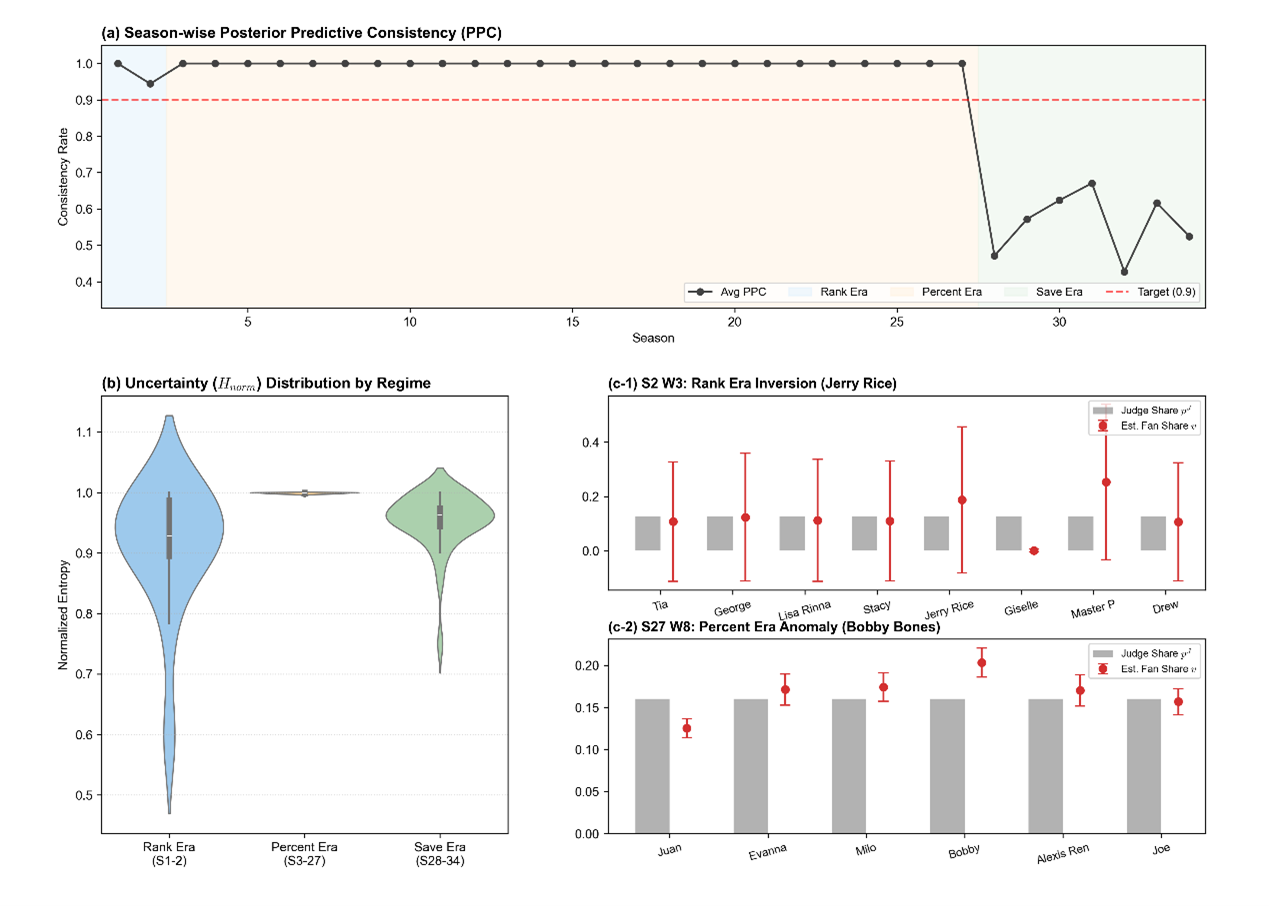
\includegraphics[width=0.62\textwidth]{figures/Q1figure2.png}
\caption{\textbf{Q1 posterior diagnostics.} (a) Season-wise PPC with regime boundaries; (b) $H_{\mathrm{norm}}(\bar{\mathbf v}_{s,t})$ by regime; (c) posterior intervals for S2W3 and S27W8 with $p^J_{i,s,t}$ overlays.}

\label{fig:q1_diag}
\end{figure}

% Gemini prompt:
% "Create a publication-style multi-panel figure titled 'Q1 Posterior Diagnostics'.
% Panel (a): line chart PPC by season (1–34), y-axis 'Mean PPC', with dashed vertical regime boundaries (1–2, 3–27a, 28a–34), annotate overall PPC=90.5%.
% Panel (b): boxplots of normalized entropy H_norm grouped by regime (Rank, Percent, Save). y-axis [0,1].
% Panel (c): two horizontal interval plots labeled 'S2 Week 3' and 'S27 Week 8'. For each, show several contestants with 95% credible intervals for vote share v; overlay judge share p^J as dots.
% Use academic font, minimal color, clean layout; no need to use real names in the mockup."

Our posterior analysis identifies distinct \textbf{Regime-Dependent Dynamics}. Season 2 (Jerry Rice) typifies judge--fan inversion where rank aggregation masks the magnitude of support, producing wider posteriors. Conversely, Season 27 (Bobby Bones) illustrates a \textbf{Systemic Anomaly} where extreme popularity concentrates posterior mass despite weak technical performance. These archetypes serve as critical stress tests for correcting anomalies without suppressing legitimate fan variance.

To facilitate downstream comparison, we export this reconstruction as a rigorous \textbf{Probabilistic Baseline}. For each week $(s,t)$, we store the full matrix of posterior draws $\mathbf V_{s,t}\in\mathbb{R}^{M\times |C_{s,t}|}$ together with derived diagnostics (credible intervals, PPC). This ensures that Q2 compares aggregation rules under identical uncertainty conditions, treating these draws as the sole admissible interface for fan support.

Finally, the analysis reveals a \textbf{Structural Separation} inherent in the Save Era, distinguishing the \emph{baseline aggregator} from the \emph{safety layer}. This insight grounds the **Modular Safety Network (MSN)** proposed in Q4: a structured composition that combines a stable percent baseline with minimal bottom-two protection, introducing fan-facing features only after establishing baseline stability.
